\section{Results}
\label{sec:results}
% We present the results in two figures, each containing several graphs. \Cref{fig:bin-time} gives graphs that plots the \emph{ID} against the number of clicks of a game
% and \Cref{fig:bin-length} gives graphs that plot the \emph{ID} against the duration of a game.
%
% The first row uses semantic distance, the second row semantic graph distance, the third row uses the graph distance, and the fourth row uses the value 1 for the distance.
% The first column uses the value 1 for the width, the second column PageRank and the third column the indegree.
% The value 1 for the width and the distance serve as a control metric to see how they influence the correlation.
% The bottem left graph is empty, since they have the value 1 for both distance and correlation, which always gives the same \emph{ID}.

We present our results in \Cref{fig:bin-length}. First, we note that some metrics gave quite good results, with three of them having $r \geq 0.84$ even over hundreds of bins. We will go over the various results we have, grouping them by the used distance metric.

\paragraph{Semantic distance}
We found that the semantic distance by itself is a poor indicator of task difficulty, with $r = 0.56$. However, by including the PageRank of the target article, results improved significantly, going up to $r = 0.84$. We believe the reason for this is that the semantic distance by itself does not take into account the graph structure, which seems to be an important factor in total task difficulty.

\paragraph{Semantic graph distance}
The results here are very good, especially without PageRank, giving $r = 0.91$. This further reaffirms our earlier belief that graph structure is important: this distance metric includes the graph structure by definition. Adding PageRank worsens our result somewhat, going down to $r = 0.87$, but results are still good. We think this is because the graph structure gets weighted too heavily by including it `twice'. (TODO: add things about other binning strategy).

\paragraph{Graph distance}
These results are very limited when we do not include PageRank, as they collapse into 5 bins. This is because there are only very few possible values here. As such the r-value of $r = 0.99$ looks nice, but is kind of `inflated' by the low number of datapoints. However, it is interesting to see that the relationship does seem to hold according to the limited information we have.

When we add PageRank, which gives us a reasonable number of bins again, we find $r = 0.80$. This is lower than the other two distance metrics. This seems to indicate that the semantic distance adds useful information about the difficulty of a task.

\paragraph{No distance}
Finally, using only PageRank as a difficulty metric gives mediocre results, with $r = 0.74$. Given that this metric only looks at the target article and not the source article, this result seems surprisingly good. However, it is still worse than most other metrics we tried, other than semantic distance which ignores the graph structure completely.


\begin{figure}[H]
  \centering
  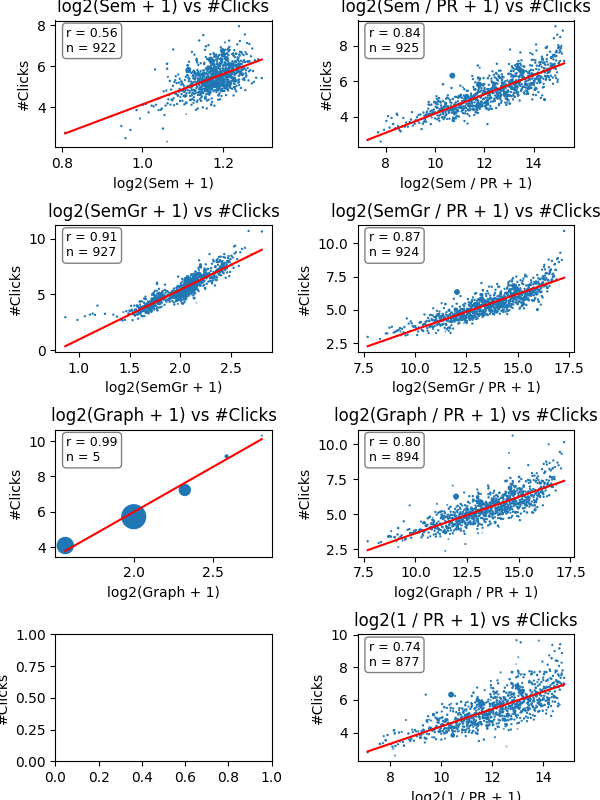
\includegraphics[width=\linewidth]{../../img/qbin-Length.png}
  \caption{Number of used clicks plotted against difficulty, using various difficulty measures and proportional binning. \\
           Left: without PageRank. Right: with PageRank. \\
           Top: `direct' semantic distance.
           Top center: `graph' semantic distance.
           Bottom center: graph distance.
           Bottom: without distance metric.}
  \label{fig:bin-length}
\end{figure}

